\chapter{Collaborative filtering}\label{chp:03-recommendationSystems}
In questo capitolo vengono approfonditi gli algoritmi di raccomandazione implementati nella soluzione proposta, mostrando alcune porzioni di 
codice e approfondendo i vari passaggi che portano a ottenere delle raccomandazioni.
%
\section{Memory-based}
I Filtri Collaborativi Memory-based determinano per l'utente, che si sta considerando, quelle raccomandazioni che sono state fatte 
ad altri utenti che la pensano allo stesso modo. Questi metodi mirano a determinare il grado o il tipo di relazione tra utenti e 
item identificando o coppie d'item che tendono a essere usati insieme o che hanno un grado di similarità alto oppure utenti 
con uno storico di item usati simile \cite{taxonomy-of-recommender-agents-on-the-internet}.
Questi approcci divennero molto famosi grazie alla loro semplicità d'implementazione, inoltre sono molto intuitivi e non necessitano di operazioni 
di training sui dati e regolazione di molti parametri, permettendo all'utente di comprendere le ragioni che si celano dietro 
ad ogni raccomandazione.\hfill\break
Questa tipologia di sistemi di raccomandazione viene definita anche Filtri Collaborativi \textit{Neighborhood-based} ed è possibile ulteriormente 
suddividerla in tre sottocategorie: User-based Filter, Item-based Filter e Hybrid Filter.
%
\subsection{User-based filtering}
Il sistema Filtraggio Collaborativo User-based, definito anche con l'acronimo UB-CF (\textit{User-based Collaborative Filter}), basa tutto il suo 
funzionamento sulla comunità di utenti, maggiore è la sua dimensione e l'attività degli utenti con item o servizi e migliori possono essere le 
raccomandazioni. Questo algoritmo fornisce dei suggerimenti a un utente sulla base di uno o più vicini (\textit{neighbours}), e la similarità 
tra utenti può essere determinata sulla base degli item che l'utente ha utilizzato o valutato.\hfill\break
Molti di questi approcci possono essere generalizzati dall'algoritmo organizzato nei seguenti passi.
\begin{enumerate}
    \item Specificare quale sia l'utente a cui si vuole applicare l'algoritmo di raccomandazione e recuperare i relativi utenti che possono 
    avere dato valutazioni o usato item simili al primo utente. Per velocizzare l'esecuzione dell'algoritmo, piuttosto che recuperare tutti 
    gli utenti, è possibile selezionare soltanto un gruppo di utenti in modo casuale oppure associare dei valori di similarità tra 
    tutti gli utenti e confrontando questi valori con quello dell'utente target, selezionare i relativi utenti che superano una soglia 
    scelta, oppure utilizzare tecniche di clustering.
    \item Estrarre gli item con cui il primo utente non ha mai interagito e per questo motivo gli possono interessare, e mostrarli 
    sotto forma di raccomandazioni.
\end{enumerate}
\begin{figure}[ht!]
    \centering
    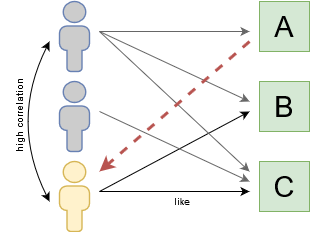
\includegraphics[scale=0.5]{images/UB_CF_ex.png}
    \caption{Esempio di applicazione di un sistema di raccomandazione User-based.}
    \label{fig:UB_CF}
\end{figure}
%
Questi approcci sono indipendenti dal contesto in cui sono applicati e possono essere più accurati rispetto 
a delle tecniche basate sul Content-based Filtering; dall'altra parte all'aumentare del numero di utenti che si considerano per 
effettuare le raccomandazioni migliore è la precisione di questo processo ma maggiore è il costo in termini di tempo.\hfill\break
Nella soluzione proposta in questa tesi, l'algoritmo UB-CF viene implementato sotto forma di funzione che prende in ingresso un parametro 
\textit{user\_other\_id}, come è possibile osservare dal Codice \ref{lst:UB_CF_1}, corrispondente all'identificativo dell'utente, 
e restituisce una lista di raccomandazioni \textit{similar\_user\_evaluations} corrispondenti alle Evaluation simili a quelle usate 
da altri utenti.\hfill\break
Per Evaluation si intende quel processo di verifica di uniformità di un certo target o asset, fornito dall'utente, a una o più politiche 
attraverso una serie di Controlli che a seconda delle caratteristiche e proprietà del target, può avere successo o meno. In altre parole, 
si può dire che un Evaluation è costituita da uno o più Controlli.
\lstset{style=python_code_style}
\begin{lstlisting}[language=Python, label=lst:UB_CF_1, caption={\ }]
# User recommendation algortihm
def user_recommendation_alg(user_other_id):
\end{lstlisting}
%
Più precisamente il funzionamento dell'algoritmo si svolge come segue.
\begin{itemize}
    \item il primo passo è quello di recuperare, sulla base del parametro in ingresso alla funzione \textit{user\_other\_id}, 
    tutte le Evaluation utilizzate dall'utente in questione;
    \begin{lstlisting}[language=Python, label=lst:UB_CF_2]
        # Select the target user and its evaluations
        target_user_evaluations = User.objects.get(other_id=user_other_id).evaluations.all()\
                                                                          .values('other_id', 'parent_id')\
                                                                          .order_by('other_id')
    \end{lstlisting}
    \item il secondo passo consiste nel selezionare le Evaluation usate dagli altri utenti, e creare una lista di queste Evaluation 
    (\textit{other\_users\_evaluations});
    \begin{lstlisting}[language=Python, label=lst:UB_CF_3]
        # Select all other users and theirs evaluations
        other_users = User.objects.exclude(other_id=user_other_id)
        # Creating a list with all the evaluations of other users
        other_users_evaluations = []
        for o_users_evaluation in other_users:
            for evaluation in o_users_evaluation.evaluations.all().values('other_id', 'parent_id').order_by('other_id'):
                other_users_evaluations.append(evaluation)
    \end{lstlisting}
    \item il terzo passo consiste nell'andare a determinare quali tra le Evaluation, dell'utente a cui si vuole raccomandare, quali sono quelle 
    simili usate dagli altri utenti. Per determinare le Evaluation simili si è andato a confrontare il parametro (\textit{parent\_id}, 
    associato ad ogni Evaluation), che identifica all'interno della base di dati quale sia il nodo padre per quella Evaluation, con lo stesso 
    parametro delle restanti Evaluation; in questo modo si è andati a selezionare soltanto gli item appartenenti a una stessa categoria, e 
    durante questo processo vengono eliminanti eventuali nodi duplicati. Infine viene composta una lista finale \textit{similar\_user\_evaluations} 
    con le Evaluation restanti.
    In definitiva ciò che ritorna questa funzione sono due liste: \textit{target\_user\_evaluations}, che contiene le Evaluation usate dall'utente 
    in questione e \textit{similar\_user\_evaluations}.
    \begin{lstlisting}[language=Python, label=lst:UB_CF_4]
        # Comparing target user's evaluations and other user's evaluations, and if there is a match the evaluation is
        # added to the 'similar_evaluations' list (the matching is made comparing the 'parent_id')
        similar_user_evaluations = []
        for t_user_evaluation in target_user_evaluations:
            for o_users_evaluation in other_users_evaluations:
                # Taking only the evaluations that have: different other_id (excluding the target evaluation
                # in the recommendation) and same parent_id and the evaluations that weren't added to 'target_user_evaluations'
                # list and to 'similar_user_evaluations'
                if ((t_user_evaluation['other_id'] != o_users_evaluation['other_id']) and  # Evaluations must have different 'other_id'
                        (t_user_evaluation['parent_id'] == o_users_evaluation['parent_id']) and  # Evaluations must have the same 'parent_id'
                        # Evaluation in all_other_evals list mustn't be already added to \
                        not (o_users_evaluation in target_user_evaluations) and  # the 'target_user_evaluations' list or
                        not (o_users_evaluation in similar_user_evaluations)):  # the 'similar_user_evaluations' list
                    similar_user_evaluations.append(o_users_evaluation)
        
        return target_user_evaluations, similar_user_evaluations
    \end{lstlisting}
\end{itemize}
%% ESEMPIO DI UNA CHIAMATA CON VALORE DI RITORNO
%\begin{figure}[ht!]
%   \centering
%   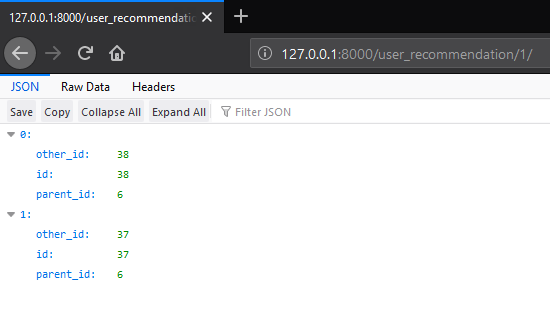
\includegraphics[scale=0.5]{images/UB_CF_test.png}
%   \caption{Esempio di una risposta in JSON a una chiamata REST all'algoritmo di raccomandazione UB-CF.}
%   \label{fig:UB_CF_resp_JSON}
%\end{figure}
Nel capitolo successivo vengono mostrati degli esempi pratici in cui è stato applicato questo algoritmo.
%
\newpage
%
\subsection{Item-based filtering}
Quando l'algoritmo UB-CF viene applicato per milioni di utenti e item non è molto efficiente per via della complessa computazione della 
ricerca di utenti simili. Per questo motivo venne ideata come alternativa il sistema Filtraggio Collaborativo Item-based, 
definito anche con l'acronimo IB-CF (\textit{Item-based Collaborative Filter}) dove si è preferito evitare di confrontare tra utenti 
simili, e al suo posto viene effettuato un confronto tra gli item dell'utente a cui si vuole raccomandare e i possibili item simili.
%
\begin{figure}[ht!]
    \centering
    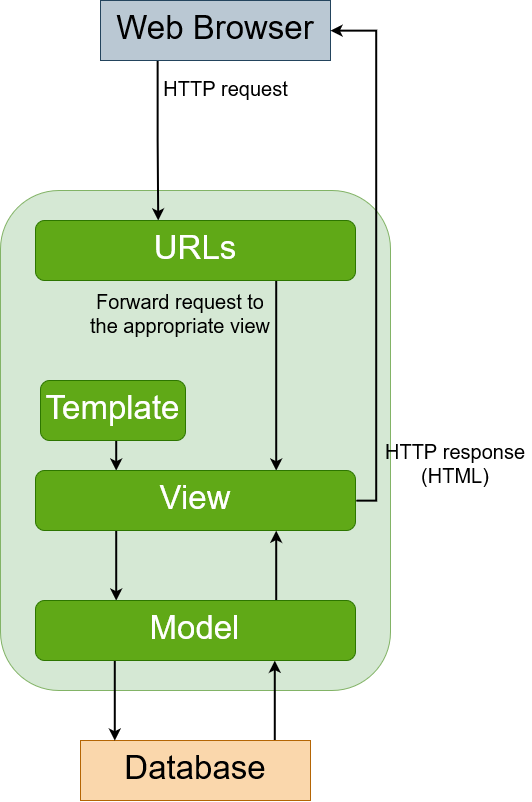
\includegraphics[scale=0.5]{images/IB_CF_ex.png}
    \caption{Esempio di applicazione di un sistema di raccomandazione IB-CF.}
    \label{fig:IB_CF}
\end{figure}
\hfill\break
Questi sistemi sono estremamente simili ai sistemi di raccomandazione Content-based, e identificano item simili in base a come sono 
stati usati dagli utenti in passato \cite{item-based-collaborative-filtering}.\hfill\break
A livello pratico nella soluzione proposta, questo algoritmo è stato implementato come funzione che ha un 
parametro \textit{item\_other\_id}, in ingresso, rappresentante l'\textit{other\_id}, un attributo associato ad ogni item all'interno della base di dati 
che lo identifica, del item su cui si vuole andare a cercare altri item simili. In generale per determinare la similarità tra due oggetti si osserva 
l'attributo \textit{parent\_id} associato a ogni item, che determina quale sia il nodo padre tra tutti i nodi all'interno del database, in sostanza 
si selezionano quegli item che appartengono alla stessa categoria.\hfill\break
In generale il IB-CF ideato per determinare Evaluation simili funziona seguendo i seguenti passi.
\begin{itemize}
    \item il primo passo è quello di recuperare sulla base del parametro in ingresso alla funzione \textit{item\_other\_id} 
    l'Evaluation su cui si vuole determinare le altre Evaluation simili;
    \begin{lstlisting}[language=Python, label=lst:IB_CF_Evaluation_1]
    def item_recommendation_alg(item_other_id):
        # Selecting the evaluation, which is applied this algorithm, from its other_id
        # SELECT * FROM recommendation_app_evaluation WHERE other_id = %(item_other_id)s AND node_type = 'eva'
        target_eval = Evaluation.objects.filter(Q(other_id=item_other_id) & Q(node_type="eva"))\
                                        .values('other_id', 'parent_id')[0]
    \end{lstlisting} 
    \item il secondo passo è quello di recuperare tutte le Evaluation, escludendo la prima recuperata, presenti nella base di dati;
    \begin{lstlisting}[language=Python, label=lst:IB_CF_Evaluation_2]
        # Selecting the other evaluations, excluding the target evaluation
        # SELECT * FROM recommendation_app_evaluation WHERE other_id != %(item_other_id)s AND node_type = 'eva'
        all_other_evals = Evaluation.objects.filter(~Q(other_id=item_other_id) & Q(node_type="eva"))\
                                        .values('other_id', 'parent_id').order_by('other_id')
    \end{lstlisting}
    \item il terzo e ultimo passo consiste nel andare a determinare le Evaluation che hanno lo stesso \textit{parent\_id}, quindi 
    quelle appartenenti alla stessa categoria, dell'Evaluation ottenuta nel primo passo; inoltre, se presenti, vengono 
    eliminati eventuali duplicati; e la funzione ritorna una lista \textit{similar\_item\_evaluations} contente le Evaluation simili.
    \begin{lstlisting}[language=Python, label=lst:IB_CF_Evaluation_3]
        # Creating a list with all the evaluations that are similar to the target evaluation (comparing the parent_id)
        similar_item_evaluations = []
        for evaluation in all_other_evals:
            # Taking only the evaluations that have: different other_id (excluding the target evaluation
            # in the recommendation) and same parent_id and the evaluations that weren't added to similar_item_evaluations
            # list
            if ((target_eval['other_id'] != evaluation['other_id']) and  # Evaluations must have different 'other_id'
                    (target_eval['parent_id'] == evaluation['parent_id']) and  # Evaluations must have same 'parent_id'
                    # Evaluation in all_other_evals list mustn't be already added to \
                    not (evaluation in similar_item_evaluations)): # the 'similar_item_evaluations' list
                similar_item_evaluations.append(evaluation)
    
    return similar_item_evaluations 
    \end{lstlisting}
\end{itemize}
%
Altro algoritmo del tipo IB-CF implementato in questa tesi sulla falsa riga di quello appena riportato nel Listing \ref{lst:IB_CF_Evaluation_1}, 
è quello ideato per determinare quali Evaluation possono essere raccomandate per un Target inserito da un utente tra quelli supportati da Moon Cloud
(Host avente Windows come sistema operativo, Host avente Linux come sistema operativo, sistemi che sfruttano 
servizi di Aws o di Azure e URL di siti web).\hfill\break
In Python questo algoritmo viene implementato come funzione che prende in ingresso l'identificativo univoco (\textit{id}) del Target, e 
restituisce l'insieme delle Evaluation raccomandate per quel Target. Il funzionamento dell'algoritmo si svolge come segue:
\begin{itemize}
    \item il primo passo è quello di recuperare tutte le Evaluation presenti nel database;
    \begin{lstlisting}[language=Python, label=lst:IB_CF_Target_1]
    def target_recommendation_alg(target_id):
        # Retriving all the evaluations in the database
        evaluations = Evaluation.objects.filter(node_type="eva")
    \end{lstlisting} 
    \item il secondo e ultimo passo è quello di andare a determinare quali sono i Controlli che hanno il valore dell'attributo \textit{target\_type\_id} 
    pari al parametro in ingresso della funzione \textit{target\_id}, e da quei Controlli determinare le Evaluation che li utilizzano, 
    eliminando eventuali duplicati; determinando così le possibili Evaluation applicabili per quel Target.
    \begin{lstlisting}[language=Python, label=lst:IB_CF_Target_2]
        # Saving in the target_evaluations list the evaluations which controls have target_type_id equal to target_id
        target_evaluations = []
        for evaluation in evaluations: # Scanning all the evaluations
            for evaluation_controls in evaluation.controls.filter(target_type_id=target_id):
                if not(evaluation in target_evaluations): # Excluding evaluations duplicated
                    target_evaluations.append(evaluation)
        
        # Converting the Evaluation model's instance in a dict and putting the evaluation, as a dict, in a list
        target_evaluations_serializer = EvaluationSerializer(target_evaluations, many=True)
        
        return target_evaluations_serializer.data
    \end{lstlisting} 
\end{itemize}
%
Nel capitolo successivo vengono mostrati anche degli esempi dei valori di risposta di queste funzioni.
%
\subsection{Hybrid Filtering} 
Nei Sistemi di Raccomandazione Ibridi si tende a voler combinare più tecniche di raccomandazione, raggruppando i 
pregi di ciascun approccio; infatti se si comparano i Sistemi di Raccomandazione Ibridi con quelli Collaborativi o 
Content-based, la precisione dei suggerimenti è solitamente maggiore.\hfill\break
Nella soluzione proposta in questa tesi, questo algoritmo viene direttamente implementato come API REST, alla quale vengono 
passati come parametri la \textit{request}, l'oggetto HTTP che il browser invia al server contenente la richiesta HTTP 
(attraverso un particolare URL) e lo \textit{user\_other\_id}, un valore recuperato come parametro dall'URL e rappresenta 
l'\textit{other\_id}, un attributo associato a ogni utente che rappresenta un identificativo per l'utente stesso. Inoltre il 
tutto viene limitato a essere richiamato solo tramite richieste HTTP con metodo GET.\hfill\break
Nel Codice \ref{lst:CF_Hybrid_Evaluation_1} si possono vedere come vengono limitate le richieste al metodo GET e come 
viene definita la funzione.
\begin{lstlisting}[language=Python, label=lst:CF_Hybrid_Evaluation_1, caption={\ }]
@api_view(['GET'])
def hybrid_recommendation(request, user_other_id)
\end{lstlisting} 
%
Il funzionamento di questo algoritmo si svolge nei seguenti passi.
\begin{itemize}
    \item il primo passo è quello di verificare se l'utente esiste nel database altrimenti viene generata un’eccezione (o errore) che è gestita in 
    modo personalizzato, generando una risposta HTTP con codice di errore 404 (Not Found);
    \begin{lstlisting}[language=Python, label=lst:CF_Hybrid_Evaluation_2]
        # Trying to retrive the actual User with user_other_id
        user = User.objects.get(other_id=user_other_id)
    \end{lstlisting} 
    \item il secondo passo è applicare l'algoritmo di User Recommandation, descritto nella sezione precendete, per le Evaluation e ottenere due liste, 
    la prima (\textit{target\_user\_evaluations}) contenente le Evaluation che l'utente ha utilizzato, mentre nella seconda (\textit{similar\_user\_evaluations}) 
    si hanno le Evaluation che gli altri utenti utilizzano e simili alle Evaluation del primo utente;
    \begin{lstlisting}[language=Python, label=lst:CF_Hybrid_Evaluation_3]
        # Taking from the user_recommendation_alg the evaluation recommended from this approach (similar_user_evaluations)
        # and the user's evaluations (target_user_evaluations)
        target_user_evaluations, similar_user_evaluations = user_recommendation_alg(user_other_id)
    \end{lstlisting} 
    \item il terzo passo consiste nell'applicazione dell'algoritmo Item-based per ogni Evaluation usata dall'utente in questione così da ottenere 
    delle raccomandazioni che sono compatibili con le Evaluation usate dall'utente; la similarità o appartenenza alla stessa categoria viene 
    ottenuta osservando il valore del \textit{parent\_id}; anche in questo caso vengono eliminati eventuali duplicati e viene formata una lista 
    (\textit{similar\_item\_evaluations}) contenente le Evaluation simili ottenute dall'applicazione dell'algoritmo di raccomandazione Item-based;
    \begin{lstlisting}[language=Python, label=lst:CF_Hybrid_Evaluation_4]
        # For every evaluation used by users is extracted all other possible evaluations that have the same 'parent_id'
        similar_item_evaluations = []
        for t_user_evaluation in target_user_evaluations:  # for every target user's evaluations
            for item_evaluation in item_recommendation_alg(t_user_evaluation['other_id']):  # is applied the item_recommendation algorithm
                # Taking only the evaluations that have: different other_id (excluding the target evaluation
                # in the recommendation) and same parent_id and the evaluations that weren't added to 'similar_item_evaluations'
                # list or to 'similar_user_evaluations' or to 'target_user_evaluations'
                if ((t_user_evaluation['other_id'] != item_evaluation['other_id']) and # Evaluations must have different 'id'
                        (t_user_evaluation['parent_id'] == item_evaluation['parent_id']) and # Evaluations must have the same 'parent_id'
                        # Evaluation in all_other_evals list mustn't be already added to \
                        not (item_evaluation in similar_item_evaluations) and # the 'similar_item_evaluations' list,
                        not (item_evaluation in similar_user_evaluations) and # the 'similar_user_evaluations' list or
                        not (item_evaluation in target_user_evaluations)): # the 'target_user_evaluations' list
                    similar_item_evaluations.append(item_evaluation)
    \end{lstlisting} 
    \item il quarto passo consiste nel raggruppare le due liste contenenti le Evaluation raccomandate per l'utente secondo l'applicazione dei 
    due algoritmi, eliminando anche eventuali duplicati, così da ottenere un'unica lista (\textit{similar\_evaluations}) la quale viene ritornata dalla 
    funzione sotto forma di risposta HTTP in formato JSON;
    \begin{lstlisting}[language=Python, label=lst:CF_Hybrid_Evaluation_5]
        # Putting together the evaluations recommended in similar_user_evaluations list and similar_item_evaluations list
        similar_evaluations = []
        # Adding to similar_evaluations list the evaluation in the similar_user_evaluations list
        for s_user_evaluation in similar_user_evaluations:
            similar_evaluations.append(s_user_evaluation)
        # Adding to similar_evaluations list the evaluation in the similar_item_evaluations list
        for item_evaluation in similar_item_evaluations:
            # Taking only the evaluations that weren't added to \
            if (not (item_evaluation in similar_evaluations) and  # the 'similar_evaluations' list or
                    not (item_evaluation in target_user_evaluations)):  # the 'target_user_evaluations' list
                similar_evaluations.append(item_evaluation)
        similar_evaluations = sorted(similar_evaluations, key=lambda i: i['other_id'])
        
        return JSONResponse(similar_evaluations, safe=False)
    \end{lstlisting} 
\end{itemize}
Nel capitolo successivo viene mostrato un esempio di risposta per quando si effettua una chiamata a questa funzione, ed è approfondito il contesto che 
è stato costruito attorno agli algoritmi di raccomandazione descritti in questo capitolo.
